\documentclass[twoside,11pt]{homework}
\usepackage{graphicx}
\usepackage{booktabs}
\usepackage{lipsum}
\usepackage{indentfirst}
\usepackage{bbm, dsfont}

\coursename{COMS 4771 Machine Learning (Spring 2015)} % DON'T CHANGE THIS

\studname{Jingwei Yang}    % YOUR NAME GOES HERE
\studmail{jy2653@columbia.edu}% YOUR UNI GOES HERE
\hwNo{2}                   % THE HOMEWORK NUMBER GOES HERE
\collab{yd2300}   % THE UNI'S OF STUDENTS YOU DISCUSSED WITH
\begin{document}
\maketitle

\section*{Problem 1}
\indent
1.  
\begin{align*}
 P_{ML} &= \arg\max\prod_{i=1}^nP^{x_{i}}(1-P)^{1-x_{i}}\\
&= \arg\max\log{\prod_{i=1}^nP^{x_{i}}(1-P)^{1-x_{i}}}\\
&= \arg\max\sum_{i=1}^n\log{P^{x_{i}}(1-P)^{1-x_{i}}}
\end{align*}

To get the maximum value, the log-likelihood maximizer must satisfy\\



\begin{align*}
0 &= \sum_{i=1}^n\nabla_P\log{P^{x_{i}}(1-P)^{1-x_{i}}} \\
&= \sum_{i=1}^n\nabla_P\log{P^{x_{i}}(1-P)^{1-x_{i}}} \\
&= \sum_{i=1}^n( \frac{x_{i}}{P} + \frac{x_{i} - 1}{1 - P})\\
&= \frac{\sum_{i=1}^nx_{i}}{P} + \frac{\sum_{i=1}^nx_{i} - n}{1-P}
\end{align*}

Solve the equation, we could get the formula of the MLE of P. 
\begin{equation}
P_{ML} =  \frac{1}{n}{\sum_{i=1}^n x_{i}}
\end{equation}



Bring $P_{ML}$ into $\sum_{i=1}^n\nabla_P\log{P^{x_{i}}(1-P)^{x_{i}}} $, we have \\
\begin{align*}
\sum_{i=1}^n\nabla_P\log{P^{x_{i}}(1-P)^{x_{i}}} &=\sum_{i=1}^n( \frac{x_{i}}{P_{ML}} + \frac{x_{i} - 1}{1 - P_{ML}}) \\
&= n + n(\frac{P_{ML} - 1}{1 - P_{ML}})\\
&= 0
\end{align*}\\


2. 
The plug-in classifier based on the BNB model is
\begin{equation}
\underset {k \in {0, 1}}{arg}\{P_k \prod_{j=1}^dP_{j,k}^{x_{j}}(1-P_{j,k})^{1-x_{j}}\} =
\underset {k \in {0, 1}}{arg}\{\log{P_k \prod_{j=1}^dP_{j,k}^{x_{j}}(1-P_{j,k})^{1-x_{j}}}\}
\end{equation}

Since there were only 2 different newsgroups, we have the classifier:
\[
f(x) =
\begin{cases} 
1 & \log{P_1 \prod_{j=1}^dP_{j,1}^{x_{j}}(1-P_{j,1})^{1-x_{j}}}  >  \log{P_2 \prod_{j=1}^dP_{j,2}^{x_{j}}(1-P_{j,2})^{1-x_{j}}} \\
2 & other
\end{cases}
\] \\

Since we have
\begin{align*}
\log{P_k \prod_{j=1}^dP_{j,k}^{x_{j}}(1-P_{j,k})^{1-x_{j}}} &= \log{P_k} + \sum_{j=1}^d x_{j} \log{P_{j,k}} + (1-x_{j})\log{(1-P_{j,k})}\\
&= \log{P_k} + \sum_{j=1}^d x_{j} \log{\frac{P_{j,k}}{1-P_{j,k}}} + \log{(1-P_{j,k})}\\
\end{align*}

Thus, 
\begin{align*}
&\log{P_1 \prod_{j=1}^dP_{j,1}^{x_{j}}(1-P_{j,1})^{1-x_{j}}}  -  \log{P_2 \prod_{j=1}^dP_{j,2}^{x_{j}}(1-P_{j,2})^{1-x_{j}}} \\
&= \log{\frac{P_{1}}{P_{2}}} + \sum_{j=1}^d x_{j} \log{\frac{P_{j,1}(1-P_{j,2})}{P_{j,2}(1-P_{j,1})}} + \log\frac{(1-P_{j,1})}{(1-P_{j,2})} \\
&= \log{\frac{P_{1}}{P_{2}}}  + \sum_{j=1}^d\log\frac{(1-P_{j,1})}{(1-P_{j,2})} + \sum_{j=1}^d x_{j} \log{\frac{P_{j,1}(1-P_{j,2})}{P_{j,2}(1-P_{j,1})}}
\end{align*}

We have classifier $f^*(x)$
\[
f^*(x) =
\begin{cases} 
1 &  \log{\frac{P_{1}}{P_{2}}}  + \sum_{j=1}^d\log\frac{(1-P_{j,1})}{(1-P_{j,2})} + \sum_{j=1}^d x_{j} \log{\frac{P_{j,1}(1-P_{j,2})}{P_{j,2}(1-P_{j,1})}} > 0\\
2 & other
\end{cases}
\] \\

Replace $\theta = - (\log{\frac{P_{1}}{P_{2}}}  + \sum_{j=1}^d\log\frac{(1-P_{j,1})}{(1-P_{j,2})})$ and $w_j = \log{\frac{P_{j,1}(1-P_{j,2})}{P_{j,2}(1-P_{j,1})}}$
, we could have 
\[
f^*(x) = 
\begin{cases} 
1 &\langle \pmb x \pmb w \rangle - \theta > 0 \\
2 & other
\end{cases}
\] \\

Thus, the plug-in classifier based on the BNB model here is a linear classifier.\\


3. The training error is 21.63 \%, and the test error is 37.6\%.
 
\section*{Problem 2}
(a)\\
if $ f_{w, \theta} (\pmb x) \neq y $\\
$\pmb w : = \pmb w + y\pmb x; \theta : = \theta - y$\\
end if

(b)\\
\begin{center}
\textbf{Learning curve on new2}\par\medskip
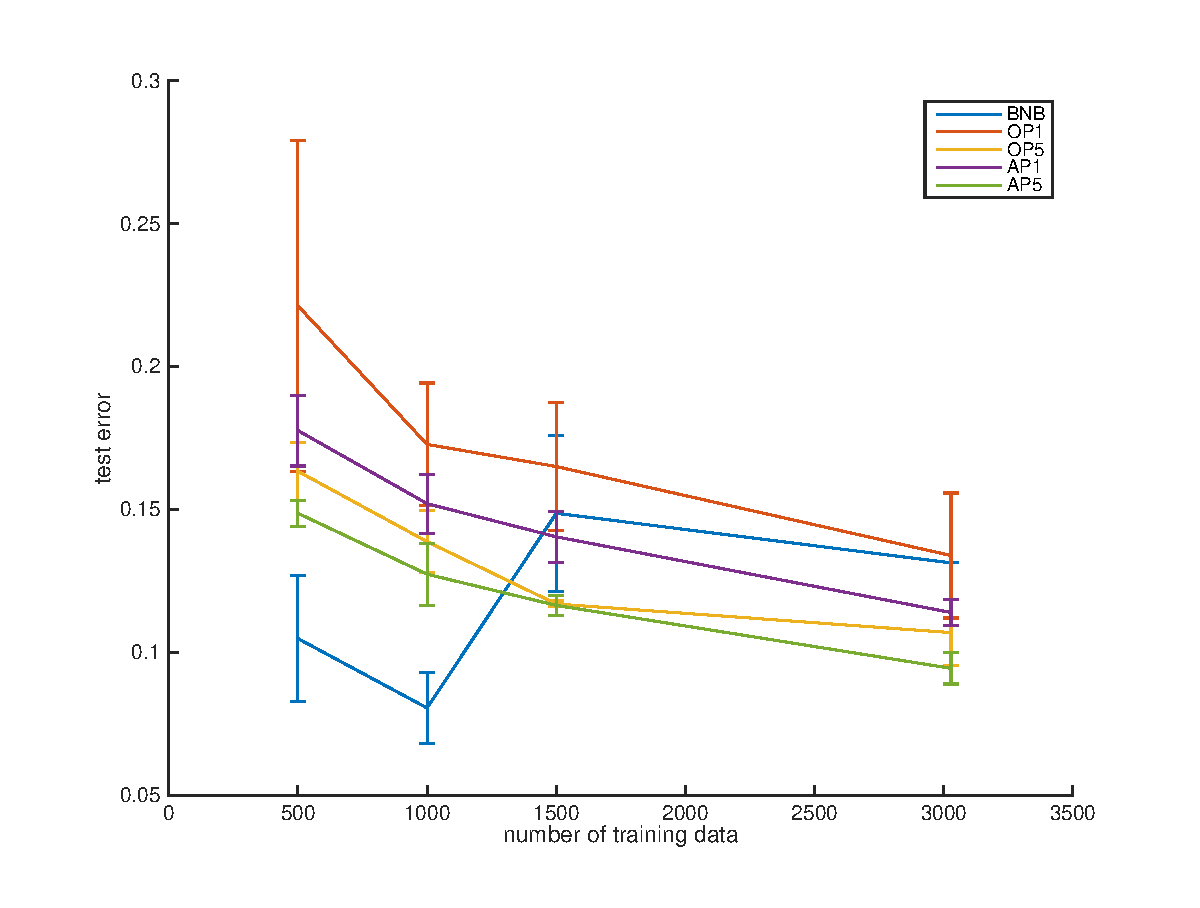
\includegraphics[width=150mm, height = 80mm]{new2.eps}
\end{center}

\begin{center}
\textbf{Learning curve on new3}\par\medskip
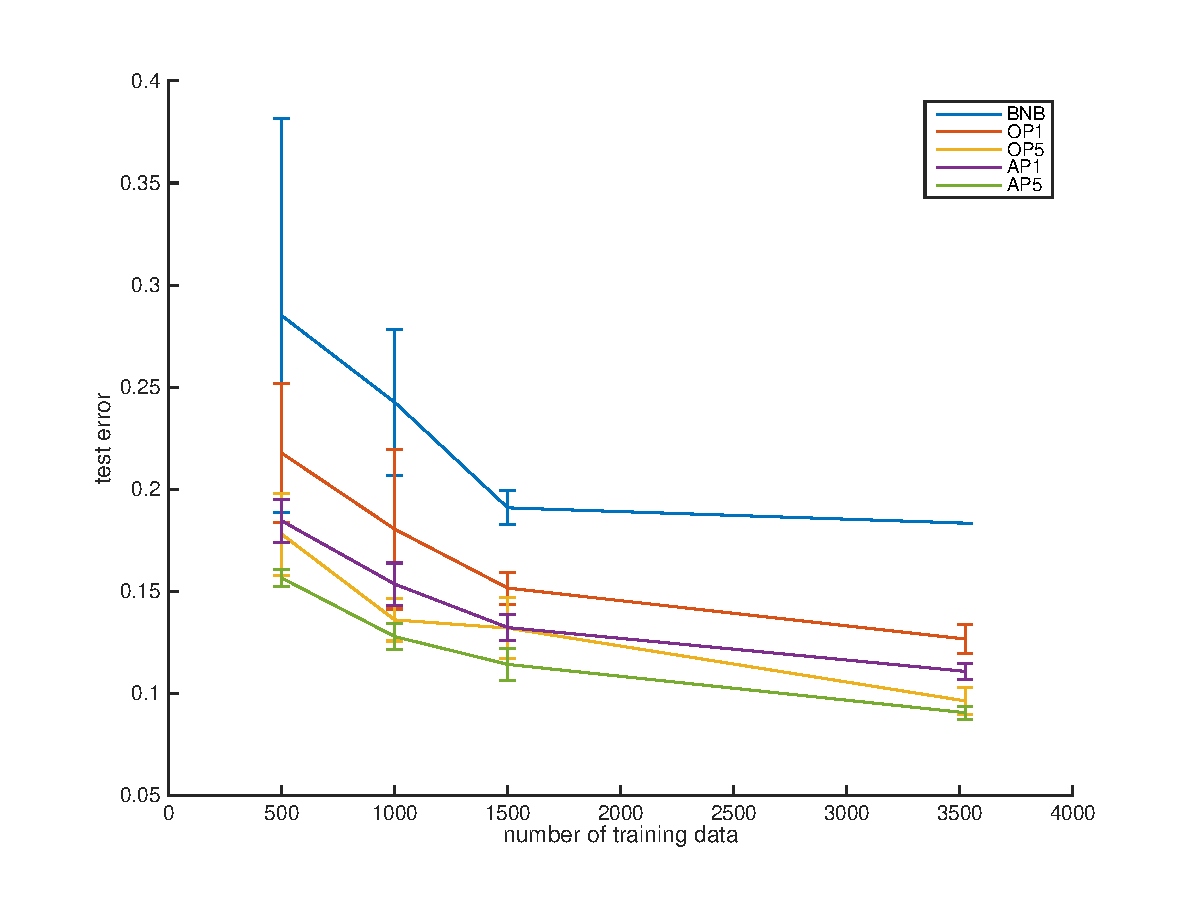
\includegraphics[width=150mm, height = 80mm]{new3.eps}
\end{center}

According to the classification result over new2 and new3. 
We could conclude that, if the the training set is large enough, the multi-pass online perceptron and average perceptron could have better classification performance over BNB classifier. 
The multi-pass perceptron could have better performance over single-pass perceptron, whether in online perceptron or average perception.  If average and online perceptron have the same times of pass, the average perception could have better performance over online perceptron. 


(c)\\
\begin{table}[h]
\caption {20 most important words} \label{tab:title}
\begin{tabular}{llllllll}

BNB\_new2    &  & BNB\_new3  &    & AP5\_new2        &  & AP5\_new3  &  \\
athos      & 5.1816 & encryption  & 5.5471 & god        & 21.7711 & windows    & 25.1524 \\
atheism    & 4.7957 & nsa         & 4.9406 & jesus      & 18.4720 & graphics   & 19.8811 \\
atheists   & 4.7642 & escrow      & 4.8818 & christian  & 18.1406 & window     & 14.4926 \\
clh        & 4.7318 & secret      & 4.8469 & gun        & 15.4042 & motif      & 14.2956 \\
firearms   & 4.6845 & pgp         & 4.8290 & bible      & 15.3759 & image      & 13.3405 \\
occupied   & 4.5487 & crypto      & 4.6750 & christians & 14.5415 & key        & 12.4873 \\
teachings  & 4.4191 & enforcement & 4.4217 & keith      & 14.3694 & space      & 11.9605 \\
israelis   & 4.4071 & government  & 4.3600 & american   & 13.3989 & win        & 11.9320 \\
serdar     & 4.3944 & motif       & 4.2610 & israel     & 13.0465 & moon       & 11.8423 \\
argic      & 4.3944 & xlib        & 4.2305 & government & 12.7633 & encryption & 11.1987 \\
ohanus     & 4.2302 & lunar       & 4.2082 & clh        & 12.3217 & circuit    & 11.1708 \\
appressian & 4.2302 & font        & 4.1814 & atheism    & 11.9379 & format     & 10.6489 \\
sahak      & 4.2302 & voltage     & 4.1599 & april      & 11.4819 & file       & 10.5748 \\
melkonian  & 4.2302 & wiretap     & 4.1599 & athos      & 11.4675 & government & 10.4239 \\
villages   & 4.2154 & xterm       & 4.1474 & lord       & 11.2899 & server     & 10.0757 \\
revelation & 4.2136 & eff         & 4.1093 & news       & 11.1809 & power      & 10.0752 \\
testament  & 4.1783 & orbit       & 4.0987 & james      & 10.8314 & large      & 9.9933  \\
livesey    & 4.1602 & denning     & 4.0920 & religious  & 10.7604 & mouse      & 9.9714  \\
atheist    & 4.1526 & sternlight  & 4.0743 & kent       & 10.7436 & low        & 9.9362  \\
solntze    & 4.1231 & vehicle     & 4.0563 & amendment  & 10.6447 & version    & 9.8288  \\
\end{tabular}
\end{table}


\section*{Problem 3}
\begin{table}[h]
\begin{tabular}{lll}
                                           & Centering  & Standardization \\
Plug-in Classifier (Gaussian Distribution) & no effects & have effects    \\
1-NN Classifier (Euclidean distance)       & no effects & have effects    \\
Greedy Decision Tree (Gini index)          & no effects & no effects      \\
ERM(Linear Classifier)                     & no effects & no effects     
\end{tabular}
\end{table}


(a)\\
a.1 Centering transformation
\begin{align*}
\hat{\pmb\mu'_{y}} &= \frac{1}{n\hat{\pi_{y}}}   \sum_{i=1}^n 1\{ {{y}_{i} = y}\}(\pmb{x}_{i} - \pmb\mu) \\
&=   \frac{1}{n\hat{\pi_{y}}}   \sum_{i=1}^n 1\{ {{y}_{i} = y}\}\pmb{x}_{i} -  \frac{1}{n\hat{\pi_{y}}}   \sum_{i=1}^n 1\{ {{y}_{i} = y}\}\pmb\mu\\
&=  \frac{1}{n\hat{\pi_{y}}}  \sum_{i=1}^n 1\{ {{y}_{i} = y}\}\pmb{x}_{i} -  \frac{1}{n\hat{\pi_{y}}} \pmb\mu\sum_{i=1}^n 1\{ {{y}_{i} = y}\}\\
&=   \frac{1}{n\hat{\pi_{y}}}  \sum_{i=1}^n 1\{ {{y}_{i} = y}\}(\pmb{x}_{i}) -    \pmb\mu
\end{align*}
Then we can plug-in the $\pmb\mu'_{y}$  into the classifer, we have:
$\pmb x' - \hat{\pmb\mu'_{y}}  = \pmb{x}- \pmb\mu - \hat{\pmb\mu_{y}} + \pmb\mu = \pmb{x} - \hat{\pmb\mu_{y}} $
 And the covariance matrix is the identity matrix \pmb I, thus the centering transformation have no effects on the resulting learning classifier.\\
 
 a.2 Standardization transformation.\\\\
 $\pmb x' - \hat{\pmb\mu'_{y}} = \frac{\pmb{x}- \pmb\mu - \hat{\pmb\mu_{y}}}{\pmb\sigma} = \frac{\pmb{x} - \hat{\pmb\mu_{y}}}{\pmb\sigma}$\\
 Since the $\sigma_i$ might not be equal to $\sigma_j$, some dimensions would be favored over other dimensions, thus the new classifier could produce different classifications. \\

(b)\\ 
Suppose we have two points: $\pmb m \in Train Set$  and $\pmb n \in Test Set$.
\begin{equation}
||\pmb m - \pmb n||_2 := \sqrt{\sum_i^d( m_i -  n_i)^2}
\end{equation}
b.1 Centering transformation. 
\begin{equation}
||\pmb m -  \pmb n||'_2 := \sqrt{\sum_i^d(m_i  - u_i - (m_i - u_i))^2}  = \sqrt{\sum_i^d( m_i -  n_i)^2} = || \pmb  m -  \pmb n||_2
\end{equation}
Thus the centering transformation have no effects over resulting learned classifier. \\

b.1 Standardization transformation. 
\begin{equation}
||\pmb m - \pmb n||'_2 := \sqrt{\sum_i^d(\frac{m_i  - u_i}{\sigma_i} - \frac{n_i  - u_i}{\sigma_i})^2}  = \sqrt{\sum_i^d \frac{1}{\sigma_i^2}( m_i -  n_i)^2} \end{equation}
Since $\sigma_i$ might be different for each dimension, some dimensions would be favored over other dimensions, thus the new classifier could produce different classifications. \\

(c)\\
c.1 Centering transformation. \\
In transformation: $\pmb x' = \pmb{x} - \pmb\mu$, $\mu_i$ is the same for $x_i$. It means all training data is shifted along the same vector $\pmb\mu$, and for any $\pmb{x}_i$, it shifts the same distance along $i$ dimension's axis. According to the definition of decision tree method, we try to find the line along $i$ dimension to minimize uncertainty. Since we just shift whole points in the same distance along each dimension, the relative position of each points is the same, the line we want find just shifts the same distance in each dimensions respectively. Therefore, the centering transformation have no effects over resulting learned classifier. \\

c.2 Standardization transformation \\
The same as the above analysis. The decision tree is constructed by drawing a line at $i$ dimension, which could minimize the uncertainty. What standardization transformation do at each dimension is to shift all points the distance of $\frac{\mu}{\sigma_i}$ and contract the factor of $\sigma_i$, the points' relative position at each dimension keep the same during this transformation. The transformation only affects the cutting line's position, but the uncertainty at the cutting line's two side keeps the same. Therefore, the standardization transformation have no effects over resulting learned classifier.\\

(d)\\
d.1 Centering transformation. \\
Linear ERM Classifier is to find the hyperplane separates the training data into two parts.  In transformation: $\pmb x' = \pmb{x} - \pmb\mu$, $\mu_i$ is the same for $x_i$. It means all training data is shifted along the same vector $\pmb\mu$, and for any $\pmb{x}_i$, it shifts the same distance along $i$ dimension's axis. Thus, each points's relative position keep the same. The new classifier would have the same classifying result as the original one. \\

d.2 Standardization transformation \\
The same as the above analysis, standardization transformation shifts all points the distance of $\frac{\mu}{\sigma_i}$ and contract the factor of $\sigma_i$, the cutting position at $i$ dimension would keep the same. Thus, the standardization transformation have no effects over resulting learned classifier.

 
\section*{Problem 4}
(a)\\
$\phi : \mathbbm{R}^d \to  \mathbbm{R}^{d+\binom{d}{2}}$\\
$\phi(x) := (x_1^2, x_2^2, ..., x_d^2, \sqrt{2}x_1x_2, \sqrt{2}x_1x_3, ..., \sqrt{2}x_1x_d, \sqrt{2}x_2x_3, ...,  \sqrt{2}x_{d-1}x_d)$\\


(b)\\
Let's assume \\

$\phi_1 (x)$ is the feature map for $K_1(x, x')$ \\
$\phi_1 : \mathbbm{R}^d \to  \mathbbm{R}^{D_1}$\\
$\phi_1 (x) := (f_1(x), f_2(x), f_3(x), ...)$\\

$\phi_2 (x)$ is the feature map for $K_2(x, x')$\\
$\phi_2 : \mathbbm{R}^d \to  \mathbbm{R}^{D_2}$\\
$\phi_2 (x) := (g_1(x), g_2(x), g_3(x), ...)$\\

We have 
\begin{align*}
K_1(x, x')K_2(x, x') &= \langle \phi_1 (x), \phi_1 (x') \rangle \langle \phi_2 (x), \phi_2 (x') \rangle \\
&= {\sum_{i=1}^{|D_1|}f_i(x)f_i(x')}{\sum_{j=1}^{|D_2|}g_j(x)g_j(x')}\\
&= {\sum_{i, j}f_i(x)f_i(x')g_j(x)g_j(x')}\\
&= {\sum_{i, j}(f_i(x)g_j(x))(f_i(x')g_j(x'))}\\
\end{align*}

Thus, we can define a feature map $\phi_3 (x)$ with a feature $c_{i,j}(x)$,  and and each pair (i, j) defined as:
$c_{i,j}(x) = f_i(x)g_j(x)$.\\
$\phi_3(x)$ is the feature map for $K_1(x, x')K_2(x, x')$\\
$\phi_3 : \mathbbm{R}^d \to  \mathbbm{R}^{D_1D_2}$\\
$\phi_3 (x) := (c_{1,1}(x), c_{1,2}(x), ... , c_{1,D_2}(x), c_{2,1}(x),..., c_{D_1,D_2}(x))$\\

Let $\phi_3 (x)$ be the feature map for $K_3(x, x')$,  $K_3(x, x') = K_1(x, x')K_2(x, x')$ is also a positive definite kernel function. 
\end{document} 